%!TEX root = main.tex
% 159 words
\chapter{Plan of Remaining Work} % (fold)
\label{cha:plan_of_remaining_work}

% Emphasize the modularity of the project, split stuff up

% contingency plans - what may go wrong? So much... FPGA too big, ARM board doesn't work, System too complex / hard to port to FPGA, not enough memory on FPGA

\section{Overview} % (fold)
\label{sec:overview}
Since the start of the project there has been a fair amount of decision changes, as the scope and challenges of the project became more clear.  The initial plan (Figure~\ref{fig:gantt1}) was unrealistic in some senses, and a revised Gantt chart \footnote{Both Gantt charts were created and modified using Gantter (http://app.gantter.com)} has been created for the remaining work (Figure~\ref{fig:gantt2}). 

A notable difference between the first and second Gantt charts is that the first made far fewer attempts to break the implementation work up.  In addition, it underestimated the time that would be required to set up the L'Imperatrice board.  Finally, more time has been allowed to do the project report, as more time should have been given to writing the interim report.

The second plan is designed to split the remaining work in such a way that there is less dependence between tasks.  If at all possible the work is modularised, so that if one section becomes unfeasible, it can be dropped without affecting the outcome of the final product greatly.


\begin{figure}[tb]
	\begin{center}
		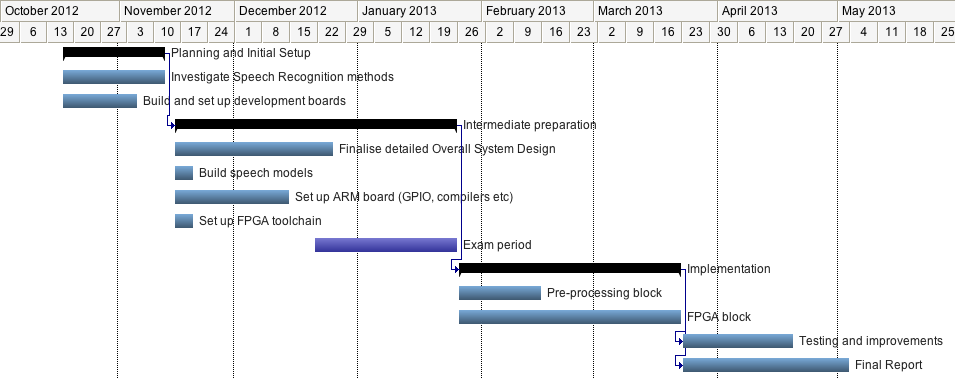
\includegraphics[width=\textwidth]{gantt-chart-initial.png}
	\end{center}
	\caption{First Gantt chart with high expectations}
	\label{fig:gantt1}
\end{figure}

\begin{figure}[tb]
	\begin{center}
		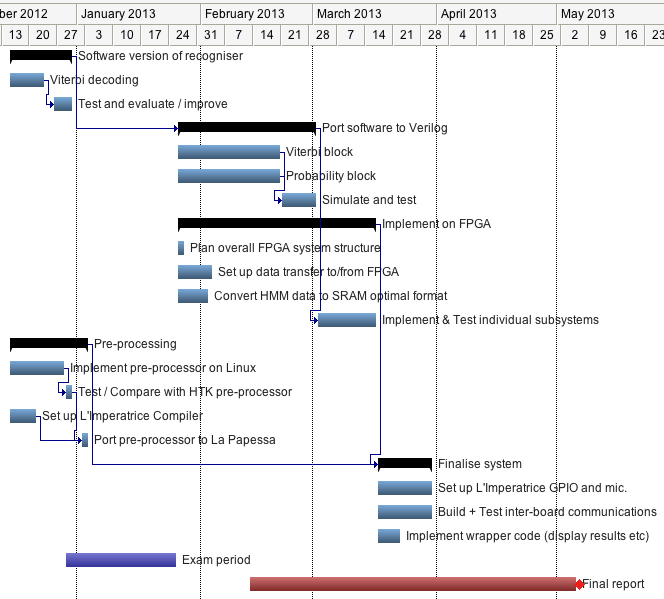
\includegraphics[width=\textwidth]{gantt-chart-interim.png}
	\end{center}
	\caption{Interim Gantt chart for remaining work}
	\label{fig:gantt2}
\end{figure}
% section overview (end)


\section{Details of tasks} % (fold) TODO
\label{sec:details_of_tasks}
The implementation of the full system requires several smaller parts,
% section details_of_tasks (end)


% chapter plan_of_remaining_work (end)